\documentclass[12pt]{article}
\newcommand{\ReportShortTitle}{Cá nhân -- Quách Gia Thịnh}
\usepackage[a4paper,top=2.1cm,bottom=2.2cm,left=2.6cm,right=2.2cm,headheight=15pt]{geometry}
\usepackage{fontspec}
\setmainfont{Times New Roman}
\setsansfont{Arial}
\setmonofont{Menlo}[Scale=0.86]
\usepackage{microtype}
\usepackage{setspace}
\setstretch{1.22}
\usepackage{parskip}
\setlength{\parindent}{1.1cm}
\setlength{\parskip}{3pt}

\usepackage{xcolor}
% Hệ màu đơn sắc: chỉ dùng đen, trắng và các mức xám để in ấn chuyên nghiệp.
\definecolor{Primary}{gray}{0}
\definecolor{Secondary}{gray}{0}
\definecolor{Accent}{gray}{0.72}
\definecolor{SoftBlue}{gray}{0.94}
\definecolor{SoftGray}{gray}{0.97}
\definecolor{Success}{gray}{0}
\definecolor{Warning}{gray}{0}
% Màu chỉ dùng bên trong khối mã nguồn.
\definecolor{CodeKeyword}{HTML}{1F4E79}
\definecolor{CodeComment}{HTML}{3F6B45}
\definecolor{CodeString}{HTML}{8A4B08}

\usepackage{graphicx}
\usepackage{booktabs}
\usepackage{longtable}
\usepackage{tabularx}
\usepackage{array}
\usepackage{makecell}
\usepackage{multirow}
\usepackage{enumitem}
\usepackage{amsmath,amssymb}
\usepackage{tikz}
\usetikzlibrary{arrows.meta,positioning,shapes.geometric,fit}
\usepackage[most]{tcolorbox}
\usepackage{listings}
\usepackage{needspace}
\renewcommand{\lstlistingname}{Đoạn mã}
\renewcommand{\lstlistlistingname}{Danh sách đoạn mã}
\renewcommand{\contentsname}{MỤC LỤC}
\usepackage{titlesec}
\usepackage{fancyhdr}
\usepackage{lastpage}
\usepackage{hyperref}
\hypersetup{colorlinks=true,linkcolor=Primary,urlcolor=Secondary,citecolor=Primary,pdfborder={0 0 0}}

\setlist[itemize]{leftmargin=1.2cm,itemsep=2pt,topsep=3pt}
\setlist[enumerate]{leftmargin=1.2cm,itemsep=2pt,topsep=3pt}
\renewcommand{\arraystretch}{1.25}
\newcolumntype{Y}{>{\raggedright\arraybackslash}X}
\newcolumntype{C}[1]{>{\centering\arraybackslash}p{#1}}
\newcolumntype{L}[1]{>{\raggedright\arraybackslash}p{#1}}

\titleformat{\section}{\Large\bfseries\color{Primary}}{\thesection.}{0.55em}{}
\titleformat{\subsection}{\large\bfseries\color{Secondary}}{\thesubsection.}{0.5em}{}
\titleformat{\subsubsection}{\normalsize\bfseries\color{Primary}}{\thesubsubsection.}{0.5em}{}
\titlespacing*{\section}{0pt}{16pt}{7pt}
\titlespacing*{\subsection}{0pt}{11pt}{5pt}

\pagestyle{fancy}
\fancyhf{}
\fancyhead[L]{\small\color{Primary}\textbf{ĐỒ ÁN ESP32-S3}}
\fancyhead[R]{\small\color{Secondary}\ReportShortTitle}
\fancyfoot[L]{\small Nhóm 3 thành viên}
\fancyfoot[R]{\small Trang \thepage/\pageref{LastPage}}
\renewcommand{\headrulewidth}{0.5pt}
\renewcommand{\footrulewidth}{0.4pt}

\newtcolorbox{summarybox}[1][Tóm tắt]{
  enhanced, breakable, colback=SoftBlue, colframe=Secondary,
  title=\textbf{#1}, coltitle=white, colbacktitle=Secondary,
  boxrule=0.7pt, arc=2mm, left=3mm, right=3mm, top=2mm, bottom=2mm
}
\newtcolorbox{evidencebox}[1][Minh chứng]{
  enhanced, breakable, colback=SoftGray, colframe=Primary,
  title=\textbf{#1}, coltitle=white, colbacktitle=Primary,
  boxrule=0.6pt, arc=1.5mm, left=3mm, right=3mm, top=2mm, bottom=2mm
}
\newtcolorbox{warningbox}[1][Lưu ý]{
  enhanced, breakable, colback=Accent!12, colframe=Warning,
  title=\textbf{#1}, coltitle=white, colbacktitle=Warning,
  boxrule=0.6pt, arc=1.5mm, left=3mm, right=3mm, top=2mm, bottom=2mm
}

\lstdefinestyle{firmware}{
  language=C++,
  basicstyle=\ttfamily\fontsize{8.35}{10.2}\selectfont,
  keywordstyle=\color{CodeKeyword}\bfseries,
  commentstyle=\color{CodeComment}\itshape,
  stringstyle=\color{CodeString},
  numbers=left,
  numberstyle=\sffamily\fontsize{6.8}{8.2}\selectfont\color{black!48},
  numbersep=9pt,
  frame=lines,
  framerule=0.45pt,
  rulecolor=\color{black!68},
  backgroundcolor=\color{white},
  framesep=5.5pt,
  breaklines=true,
  breakatwhitespace=false,
  breakindent=1.25em,
  columns=fullflexible,
  keepspaces=true,
  showstringspaces=false,
  tabsize=2,
  escapeinside={(*@}{@*)},
  xleftmargin=1.1em,
  xrightmargin=0.25em,
  framexleftmargin=1.0em,
  framexrightmargin=0.45em,
  aboveskip=9pt,
  belowskip=10pt,
  abovecaptionskip=6pt,
  belowcaptionskip=0pt,
  captionpos=b
}

% Chú thích tiếng Việt được render bằng XeLaTeX ngay trong khung mã.
\newcommand{\VNCodeComment}[1]{%
  \parbox[t]{0.93\linewidth}{%
    \raggedright\color{CodeComment}\sffamily\fontsize{7.7}{9.1}\selectfont\itshape
    \textcolor{CodeComment}{\textbf{//}}\enspace #1}%
}

\newcommand{\ProjectTitle}{THIẾT BỊ ĐEO THEO DÕI SỨC KHỎE, PHÁT HIỆN TÉ NGÃ VÀ ĐỊNH VỊ DÙNG ESP32-S3}
\newcommand{\GroupMembers}{Phạm Hùng Tiến -- Hồ Sĩ Phú -- Quách Gia Thịnh}
\newcommand{\ReportDate}{Tháng 8 năm 2026}
\newcommand{\RepositoryURL}{https://github.com/PhamHungTien/esp32-s3-health-monitor}
\newcommand{\RepositoryDisplay}{github.com/PhamHungTien/esp32-s3-health-monitor}
\newcommand{\UniversityName}{TRƯỜNG ĐẠI HỌC KHOA HỌC TỰ NHIÊN}
\newcommand{\UniversitySystem}{ĐẠI HỌC QUỐC GIA THÀNH PHỐ HỒ CHÍ MINH}
\newcommand{\FacultyName}{KHOA ĐIỆN TỬ -- VIỄN THÔNG}

\newcommand{\CoverInstitution}{%
  \centering
  
\includegraphics[height=2.8cm]{assets/branding/hcmus_logo_user.png}\par
  \vspace{0.2cm}
  {\sffamily\bfseries\small\color{Primary}\UniversitySystem\par}
  \vspace{2pt}
  {\sffamily\bfseries\fontsize{16}{20}\selectfont\color{Primary}\UniversityName\par}
  \vspace{3pt}
  {\sffamily\bfseries\large\color{Secondary}\FacultyName\par}
  \vspace{0.35cm}
  {\color{Primary}\rule{0.84\textwidth}{1.0pt}\par}
}

\newcommand{\CoverBands}{%
  \begin{tikzpicture}[remember picture,overlay]
    \fill[Primary] (current page.north west) rectangle ([yshift=-4.5mm]current page.north east);
    \fill[Secondary] (current page.south west) rectangle ([yshift=3mm]current page.south east);
  \end{tikzpicture}%
}

\newcommand{\CoverField}[2]{%
  \noindent
  \begin{minipage}[t]{0.35\linewidth}
    \raggedright\strut\sffamily\bfseries\color{Primary}#1
  \end{minipage}\hfill
  \begin{minipage}[t]{0.61\linewidth}
    \raggedright\strut\sffamily\color{black}#2
  \end{minipage}\par
}

\hypersetup{
  pdftitle={\ProjectTitle\space -- \ReportShortTitle},
  pdfauthor={\GroupMembers},
  pdfsubject={Báo cáo đồ án thiết bị theo dõi sức khỏe dùng ESP32-S3},
  pdfkeywords={ESP32-S3, MAX30102, OLED, IMU, GPS, nhịp tim, SpO2, té ngã}
}

\newcommand{\MakeReportCover}[4]{%
  \hypersetup{pageanchor=false}
  \begin{titlepage}
    \thispagestyle{empty}
    \centering
    \CoverBands
    \vspace*{0.05cm}
    \CoverInstitution
    \vspace{0.45cm}
    {\sffamily\bfseries\normalsize\color{Secondary} BÁO CÁO ĐỒ ÁN\par}
    \vspace{0.35cm}
    {\sffamily\bfseries\fontsize{18}{23}\selectfont\color{Primary}\ProjectTitle\par}
    \vspace{0.6cm}
    \begin{tcolorbox}[width=0.84\textwidth,colback=SoftBlue,colframe=Secondary,arc=1.8mm,boxrule=0.8pt,left=4mm,right=4mm,top=2.7mm,bottom=2.7mm]
      \centering{\sffamily\bfseries\normalsize\color{Secondary} #1\par}
    \end{tcolorbox}
    \vfill
    \begin{tcolorbox}[width=0.84\textwidth,colback=white,colframe=Primary!48,arc=1.2mm,boxrule=0.6pt,left=6mm,right=6mm,top=4.5mm,bottom=4.5mm]
      \raggedright
      \CoverField{Người thực hiện}{#2}
      \vspace{2.1mm}
      \CoverField{Mã số sinh viên}{#3}
      \vspace{2.1mm}
      \CoverField{Nhóm}{03 thành viên}
      \vspace{2.1mm}
      \CoverField{Phạm vi báo cáo}{#4}
    \end{tcolorbox}
    \vfill
    {\sffamily\footnotesize\color{Secondary}\GroupMembers\par}
    \vspace{0.2cm}
    {\sffamily\footnotesize\color{Primary}\textbf{Mã nguồn đồ án: }
      \href{\RepositoryURL}{\RepositoryDisplay}\par}
    \vspace{0.2cm}
    {\sffamily\bfseries\small\color{Primary}Thành phố Hồ Chí Minh, \ReportDate\par}
    \vspace{0.2cm}
  \end{titlepage}
  \hypersetup{pageanchor=true}
  \clearpage
}

\newcommand{\MakeGroupCover}[1]{%
  \hypersetup{pageanchor=false}
    \begin{titlepage}
    \thispagestyle{empty}
    \centering
    \CoverBands
    \vspace*{0.05cm}
    \CoverInstitution
    \vspace{0.45cm}
    {\sffamily\bfseries\normalsize\color{Secondary} BÁO CÁO ĐỒ ÁN\par}
    \vspace{0.35cm}
    {\sffamily\bfseries\fontsize{18}{23}\selectfont\color{Primary}\ProjectTitle\par}
    \vspace{0.6cm}
    \begin{tcolorbox}[width=0.84\textwidth,colback=SoftBlue,colframe=Secondary,arc=1.8mm,boxrule=0.8pt,left=4mm,right=4mm,top=2.7mm,bottom=2.7mm]
      \centering{\sffamily\bfseries\normalsize\color{Secondary} #1\par}
    \end{tcolorbox}
    \vfill
    \begin{tcolorbox}[width=0.84\textwidth,colback=white,colframe=Primary!48,arc=1.2mm,boxrule=0.6pt,left=6mm,right=6mm,top=4.5mm,bottom=4.5mm]
      \sffamily
      {\bfseries\color{Primary}THÀNH VIÊN THỰC HIỆN\par}
      \vspace{3mm}
      \begin{tabularx}{\linewidth}{C{1.1cm} Y C{3.0cm}}
        \toprule
        \textbf{STT} & \textbf{Họ và tên} & \textbf{MSSV}\\
        \midrule
        1 & Phạm Hùng Tiến & 24207043\\
        2 & Hồ Sĩ Phú & 24207101\\
        3 & Quách Gia Thịnh & 24207105\\
        \bottomrule
      \end{tabularx}
    \end{tcolorbox}
    \vfill
    {\sffamily\footnotesize\color{Primary}\textbf{Mã nguồn đồ án: }
      \href{\RepositoryURL}{\RepositoryDisplay}\par}
    \vspace{0.2cm}
    {\sffamily\bfseries\small\color{Primary}Thành phố Hồ Chí Minh, \ReportDate\par}
    \vspace{0.2cm}
  \end{titlepage}
  \hypersetup{pageanchor=true}
  \clearpage
}

\newcommand{\Code}[1]{\texttt{#1}}
\newcommand{\OK}{\textcolor{Success}{\textbf{Đạt}}}
\newcommand{\Implemented}{\textcolor{Secondary}{\textbf{Đã cài đặt}}}
\newcommand{\NeedTest}{\textcolor{Warning}{\textbf{Cần thử thêm}}}
\newcommand{\Pending}{\textcolor{Warning}{\textbf{Cần hiệu chuẩn}}}


\begin{document}
\MakeReportCover{BÁO CÁO CÔNG VIỆC CÁ NHÂN}{Quách Gia Thịnh}{24207105}{Phát hiện té ngã, đếm bước, định vị GPS và luồng cảnh báo}

\begin{summarybox}[Nội dung phụ trách]
Trong đồ án, em phụ trách đọc dữ liệu IMU, đếm bước, phát hiện té ngã, nhận dữ liệu GPS qua UART và tách thông tin vị trí từ các câu NMEA.
\end{summarybox}

\section{Mục tiêu công việc}

Chức năng té ngã cần phân biệt va chạm thông thường với chuỗi rơi--va đập--bất động. Phần GPS phải nhận liên tục dữ liệu NMEA, kiểm tra checksum và phân biệt được trạng thái chưa có tín hiệu, chưa có vị trí và đã bắt được tọa độ.

\section{Mô-đun IMU, đếm bước và té ngã}

\subsection{Khởi tạo và chuẩn hóa}

Thiết bị I2C tại 0x68 trả về \Code{WHO\_AM\_I=0x74}. Em đọc sáu byte dữ liệu của các trục $x,y,z$, đổi sang đơn vị $g$ và tính độ lớn:

\begin{center}
\small
\begin{tabularx}{0.90\textwidth}{C{2.1cm} C{2.0cm} Y}
\toprule
\textbf{Thanh ghi} & \textbf{Giá trị} & \textbf{Mục đích}\\
\midrule
0x75 & chỉ đọc & Kiểm tra mã \Code{WHO\_AM\_I}\\
0x6B & 0x00 & Đưa IMU ra khỏi chế độ ngủ\\
0x1C & 0x00 & Chọn thang gia tốc $\pm 2g$\\
0x1A & 0x03 & Bật bộ lọc số mức 3\\
0x3B & đọc 6 byte & Lấy liên tiếp $a_x,a_y,a_z$\\
\bottomrule
\end{tabularx}
\normalsize
\end{center}

\[
 A=\sqrt{a_x^2+a_y^2+a_z^2}.
\]

Ở trạng thái đặt yên, phép đo thực tế đạt khoảng 1,07--1,08$g$, phù hợp với gia tốc trọng trường và được dùng làm mốc bất động.

\subsection{Máy trạng thái phát hiện té ngã}

Em triển khai bốn trạng thái để kiểm tra đầy đủ diễn biến của một lần té ngã:

\begin{enumerate}
  \item \textbf{NORMAL:} theo dõi bình thường;
  \item \textbf{FREEFALL:} xác nhận gia tốc thấp trong một khoảng ngắn;
  \item \textbf{IMPACT:} chờ va đập mạnh trong cửa sổ thời gian giới hạn;
  \item \textbf{ALERT:} chỉ kích hoạt sau khi có giai đoạn ít chuyển động sau va đập.
\end{enumerate}

Mọi trạng thái trung gian đều có timeout để quay về NORMAL nếu chuỗi sự kiện không hoàn chỉnh. Cấu trúc này loại nhiều báo giả do vung tay hoặc đặt thiết bị mạnh xuống bàn.

\Needspace{0.42\textheight}
\thispagestyle{fancy}
\begin{lstlisting}[style=firmware,caption={Các điều kiện quyết định trong máy trạng thái té ngã}]
case FALL_NORMAL:
  if (accelerationG < 0.45f) {
    if (lowGStartMs == 0) lowGStartMs = now;
    if (now - lowGStartMs >= 120) {
      fallState = FALL_FREE_FALL;
      fallStateMs = now;
    }
  } else {
    lowGStartMs = 0;
  }
  if (accelerationG > 2.8f) {
    fallState = FALL_IMPACT;
    fallStateMs = now;
  }
  break;

case FALL_IMPACT:
  if (now - fallStateMs > 1800 && motionLevel < 0.08f &&
      accelerationG > 0.72f && accelerationG < 1.28f) {
    fallState = FALL_ALERT;
    fallStateMs = now;
  } else if (now - fallStateMs > 5000) {
    fallState = FALL_NORMAL;
  }
  break;
\end{lstlisting}

\begin{codeexplanation}
\CodeExplainLine{1}{Bắt đầu nhánh xử lý khi máy trạng thái đang ở điều kiện vận động bình thường.}
\CodeExplainLine{2}{Kiểm tra tổng gia tốc nhỏ hơn 0,45 g, dấu hiệu cơ thể có thể đang rơi tự do.}
\CodeExplainLine{3}{Lưu mốc bắt đầu mức gia tốc thấp nếu đây là mẫu thấp đầu tiên.}
\CodeExplainLine{4}{Yêu cầu điều kiện gia tốc thấp kéo dài ít nhất 120 ms để loại nhiễu tức thời.}
\CodeExplainLine{5}{Chuyển máy trạng thái sang giai đoạn rơi tự do đã được xác nhận.}
\CodeExplainLine{6}{Lưu thời điểm chuyển trạng thái để kiểm soát thời hạn của giai đoạn tiếp theo.}
\CodeExplainLine{7}{Kết thúc khối xác nhận đủ thời gian gia tốc thấp.}
\CodeExplainLine{8}{Đi vào nhánh này khi tổng gia tốc đã trở lại từ 0,45 g trở lên.}
\CodeExplainLine{9}{Xóa mốc gia tốc thấp vì chuỗi rơi tự do không còn liên tục.}
\CodeExplainLine{10}{Kết thúc phép kiểm tra rơi tự do.}
\CodeExplainLine{11}{Kiểm tra xung va đập trực tiếp lớn hơn 2,8 g.}
\CodeExplainLine{12}{Chuyển sang trạng thái va đập khi phát hiện xung mạnh.}
\CodeExplainLine{13}{Lưu thời điểm va đập để bắt đầu cửa sổ kiểm tra bất động.}
\CodeExplainLine{14}{Kết thúc nhánh phát hiện va đập trực tiếp.}
\CodeExplainLine{15}{Thoát khỏi nhánh trạng thái bình thường của câu lệnh switch.}
\CodeExplainLine{16}{Dòng trống phân tách hai trạng thái của máy trạng thái.}
\CodeExplainLine{17}{Bắt đầu nhánh xử lý sau khi đã phát hiện va đập.}
\CodeExplainLine{18}{Yêu cầu đã qua 1.800 ms và mức chuyển động nhỏ hơn 0,08 g.}
\CodeExplainLine{19}{Đồng thời yêu cầu tư thế tĩnh có tổng gia tốc gần 1 g, trong khoảng 0,72--1,28 g.}
\CodeExplainLine{20}{Chuyển sang cảnh báo té ngã khi toàn bộ điều kiện bất động đều đúng.}
\CodeExplainLine{21}{Lưu thời điểm phát cảnh báo để phục vụ hiển thị, còi và thao tác hủy.}
\CodeExplainLine{22}{Nếu sau 5 giây vẫn không đủ điều kiện bất động thì xem va đập là sự kiện giả.}
\CodeExplainLine{23}{Đưa máy trạng thái về bình thường để tiếp tục giám sát.}
\CodeExplainLine{24}{Kết thúc nhánh hết thời hạn chờ sau va đập.}
\CodeExplainLine{25}{Thoát khỏi nhánh trạng thái va đập.}
\end{codeexplanation}

\subsection{Đếm bước}

Độ lớn gia tốc được tách thành thành phần nền và thành phần chuyển động. Một đỉnh chỉ được xem là bước khi vượt ngưỡng, cách đỉnh trước ít nhất 280 ms và nằm trong chuỗi có chu kỳ không quá 1,8 giây. Bước đầu tiên chỉ được cộng sau khi xuất hiện đỉnh thứ hai, nhờ đó việc cầm thiết bị lên không làm tăng bộ đếm.

\Needspace{0.38\textheight}
\begin{lstlisting}[style=firmware,caption={Lọc gia tốc động và xác nhận chuỗi bước}]
gravity += 0.03f * (totalG - gravity);
float dynamicG = totalG - gravity;
dynamicFiltered += 0.25f * (dynamicG - dynamicFiltered);

if (dynamicFiltered < -0.05f) peakArmed = true;
if (peakArmed && dynamicFiltered > 0.11f &&
    now - lastPeakMs > 280 && totalG < 1.8f) {
  uint32_t interval = lastPeakMs == 0 ? 0 : now - lastPeakMs;
  if (interval >= 280 && interval <= 1800) {
    if (walkingSequence) {
      stepCount++;
    } else {
      stepCount += 2;
      walkingSequence = true;
    }
  } else {
    walkingSequence = false;
  }
  lastPeakMs = now;
  peakArmed = false;
}
\end{lstlisting}

\begin{codeexplanation}
\CodeExplainLine{1}{Cập nhật thành phần trọng lực bằng bộ lọc thông thấp với hệ số 0,03.}
\CodeExplainLine{2}{Loại thành phần trọng lực khỏi tổng gia tốc để thu phần gia tốc do bước chân.}
\CodeExplainLine{3}{Lọc tiếp gia tốc động với hệ số 0,25 để giảm nhiễu cao tần.}
\CodeExplainLine{4}{Dòng trống phân tách bước lọc tín hiệu với bước phát hiện một chu kỳ bước.}
\CodeExplainLine{5}{Mở cờ chờ đỉnh dương sau khi tín hiệu đã đi qua đáy âm nhỏ hơn -0,05 g.}
\CodeExplainLine{6}{Yêu cầu tín hiệu vượt đỉnh dương 0,11 g khi cờ chờ đã được mở.}
\CodeExplainLine{7}{Giữ khoảng cách tối thiểu 280 ms giữa hai đỉnh và loại xung mạnh từ 1,8 g trở lên.}
\CodeExplainLine{8}{Tính khoảng giữa hai đỉnh; đặt bằng 0 nếu chưa từng có đỉnh trước đó.}
\CodeExplainLine{9}{Chấp nhận nhịp bước có chu kỳ từ 280 đến 1.800 ms.}
\CodeExplainLine{10}{Kiểm tra chuỗi đi bộ đã được xác nhận từ một cặp đỉnh trước hay chưa.}
\CodeExplainLine{11}{Khi chuỗi đã hợp lệ, mỗi đỉnh mới làm tăng bộ đếm thêm một bước.}
\CodeExplainLine{12}{Đi vào nhánh khởi tạo khi vừa thu được cặp đỉnh hợp lệ đầu tiên.}
\CodeExplainLine{13}{Cộng hai bước cùng lúc để bù cho đỉnh đầu tiên chưa được tính trước khi xác nhận chuỗi.}
\CodeExplainLine{14}{Đánh dấu hệ thống đang trong một chuỗi đi bộ hợp lệ.}
\CodeExplainLine{15}{Kết thúc nhánh lựa chọn cách cộng bước.}
\CodeExplainLine{16}{Đi vào nhánh này khi khoảng đỉnh nằm ngoài miền nhịp bước cho phép.}
\CodeExplainLine{17}{Hủy trạng thái chuỗi đi bộ để lần kế tiếp phải xác nhận lại.}
\CodeExplainLine{18}{Kết thúc kiểm tra khoảng thời gian giữa hai đỉnh.}
\CodeExplainLine{19}{Lưu mốc đỉnh hiện tại cho phép tính khoảng đỉnh ở lần sau.}
\CodeExplainLine{20}{Đóng cờ chờ đỉnh, buộc tín hiệu phải qua một đáy âm mới trước bước tiếp theo.}
\CodeExplainLine{21}{Kết thúc điều kiện xác nhận đỉnh dương.}
\end{codeexplanation}

\section{Mô-đun định vị GPS}

\subsection{UART và thu dữ liệu}

GPS hoạt động ở 9600 baud trên một UART phần cứng riêng. Sau khi thay lại dây đúng chiều tín hiệu, bộ đếm đã nhận hơn 7.000 byte NMEA liên tục. Việc đọc UART nằm trong mọi vòng lặp để không tràn bộ đệm. Phần thu dòng, checksum và parser được viết trực tiếp, không dùng TinyGPS++ hoặc thư viện GPS bên ngoài.

\begin{figure}[htbp]
  \centering
  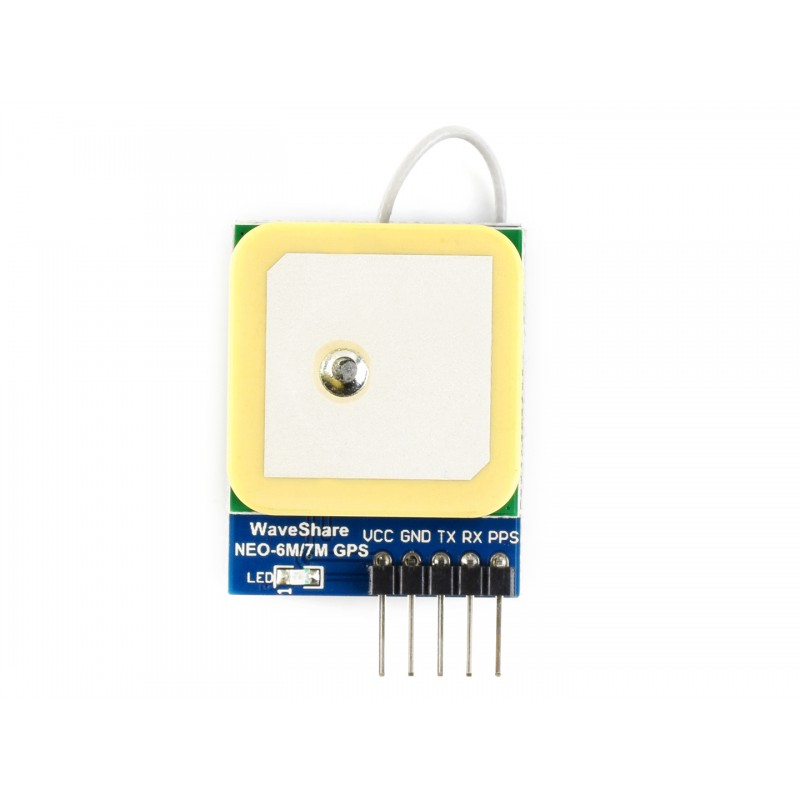
\includegraphics[width=0.34\textwidth,height=4.2cm,keepaspectratio,trim=180 55 180 55,clip]{assets/components/gps_neo6m_reference.jpg}
  \caption{Mô-đun GPS UART tham chiếu. Đồ án xác nhận khối định vị bằng dữ liệu NMEA 9600 baud; cần thay ảnh nếu nhãn mô-đun thật khác. Nguồn: \href{https://www.waveshare.com/uart-gps-neo-6m.htm}{Waveshare}.}
  \label{fig:thinh-gps}
\end{figure}

\subsection{Kiểm tra và giải mã NMEA}

Em gom dữ liệu từ ký tự ``\$'' đến cuối dòng, tính XOR phần thân và so sánh với checksum sau dấu ``*''. Chỉ câu đúng checksum mới được tách trường. Câu GGA cung cấp chất lượng fix, số vệ tinh và vị trí; câu RMC cho biết bản tin vị trí có hợp lệ hay không.

Vĩ độ/kinh độ từ dạng độ--phút được đổi sang độ thập phân:

\[
 d_{decimal}=d+\frac{m}{60},
\]

và đổi dấu cho bán cầu Nam hoặc Tây. Vị trí chỉ được đánh dấu FIX khi câu hợp lệ báo chất lượng tốt, ký hiệu bán cầu đúng và tọa độ nằm trong miền cho phép. Khi bản tin mới báo mất fix, trạng thái chuyển sang NOFIX; tọa độ hợp lệ gần nhất vẫn được giữ riêng để dùng trong màn hình cảnh báo.

\Needspace{0.34\textheight}
\begin{lstlisting}[style=firmware,caption={Tính và kiểm tra checksum NMEA trước khi tách trường}]
bool NMEA_ChecksumOK(const char *sentence) {
  if (!sentence || sentence[0] != '$') return false;
  const char *star = strchr(sentence, '*');
  if (!star || strlen(star) < 3) return false;
  int8_t high = NMEA_HexNibble(star[1]);
  int8_t low = NMEA_HexNibble(star[2]);
  if (high < 0 || low < 0) return false;

  uint8_t checksum = 0;
  for (const char *p = sentence + 1; p < star; p++) {
    checksum ^= (uint8_t)*p;
  }
  uint8_t expected = (uint8_t)((high << 4) | low);
  return checksum == expected;
}
\end{lstlisting}

\begin{codeexplanation}
\CodeExplainLine{1}{Khai báo hàm kiểm tra checksum và nhận chuỗi NMEA dạng ký tự làm đầu vào.}
\CodeExplainLine{2}{Loại con trỏ rỗng hoặc chuỗi không bắt đầu bằng ký tự đô-la theo chuẩn NMEA.}
\CodeExplainLine{3}{Tìm dấu sao, vị trí phân cách phần dữ liệu với hai chữ số checksum.}
\CodeExplainLine{4}{Loại câu không có dấu sao hoặc không đủ hai ký tự checksum phía sau.}
\CodeExplainLine{5}{Đổi chữ số hexadecimal thứ nhất sau dấu sao thành bốn bit cao.}
\CodeExplainLine{6}{Đổi chữ số hexadecimal thứ hai thành bốn bit thấp.}
\CodeExplainLine{7}{Loại câu có một trong hai chữ số checksum không hợp lệ.}
\CodeExplainLine{8}{Dòng trống phân tách bước đọc checksum nhận được với bước tự tính checksum.}
\CodeExplainLine{9}{Khởi tạo biến checksum tính toán bằng 0.}
\CodeExplainLine{10}{Duyệt các ký tự sau dấu đô-la và dừng ngay trước dấu sao.}
\CodeExplainLine{11}{XOR từng byte vào biến tích lũy đúng theo quy tắc checksum NMEA.}
\CodeExplainLine{12}{Kết thúc vòng lặp sau khi đã xử lý toàn bộ phần thân câu.}
\CodeExplainLine{13}{Ghép bốn bit cao và bốn bit thấp thành byte checksum nhận được.}
\CodeExplainLine{14}{Chỉ chấp nhận câu khi checksum tự tính bằng checksum đi kèm.}
\CodeExplainLine{15}{Kết thúc thân hàm.}
\end{codeexplanation}

\subsection{Trạng thái vận hành}

\begin{itemize}
  \item \textbf{WAIT:} chưa nhận byte GPS;
  \item \textbf{LOST:} từng nhận nhưng mất dữ liệu quá 3 giây;
  \item \textbf{NOFIX:} đang nhận NMEA nhưng chưa có vị trí;
  \item \textbf{FIX:} có tọa độ hợp lệ gần thời điểm hiện tại.
\end{itemize}

\section{Nhật ký khối lượng}

\begin{tabularx}{\textwidth}{L{7.5cm} C{2.2cm} Y}
\toprule
\textbf{Hạng mục} & \textbf{Thời lượng} & \textbf{Đầu ra}\\
\midrule
Khởi tạo, đọc và chuẩn hóa IMU & 5 giờ & $a_x,a_y,a_z,A$ theo đơn vị $g$\\
Lọc chuyển động và đếm bước & 4 giờ & Mức chuyển động, số bước\\
Máy trạng thái té ngã & 7 giờ & FREEFALL--IMPACT--ALERT\\
Cấu hình UART và kiểm tra luồng GPS & 4 giờ & Dòng NMEA 9600 baud\\
Checksum, bộ đệm và parser GGA/RMC & 6 giờ & Vị trí, vệ tinh, trạng thái fix\\
Tích hợp vị trí vào cảnh báo, kiểm thử & 4 giờ & Dữ liệu cảnh báo hoàn chỉnh\\
\midrule
\textbf{Tổng} & \textbf{30 giờ} & \textbf{Đã cài đặt; cần thử đối chứng}\\
\bottomrule
\end{tabularx}

\section{Kết quả kiểm thử}

\begin{tabularx}{\textwidth}{L{4.4cm} L{5.1cm} Y}
\toprule
\textbf{Nội dung} & \textbf{Kết quả quan sát} & \textbf{Đánh giá}\\
\midrule
Định danh IMU & WHO\_AM\_I = 0x74 & \OK\\
Gia tốc nghỉ & 1,07--1,08$g$ & \OK\\
Đếm bước khi đặt yên & Giữ nguyên 0, không tự tăng & \OK\\
Đếm bước với dữ liệu tổng hợp & 20 chu kỳ chuyển động cho kết quả 20 bước; nhiễu nhỏ và một rung đơn cho 0 bước & \OK\\
Đếm bước khi đi bộ & Đã có thuật toán; chưa thu đủ số bước chuẩn để tính sai số & \NeedTest\\
UART GPS & Bộ đếm byte tăng liên tục & \OK\\
GPS ngoài trời/gần cửa sổ & FIX, 4 vệ tinh ở lần chạy cuối, có tọa độ & \OK\\
GPS khi tín hiệu kém & NOFIX, không tạo tọa độ mới & \OK\\
Máy trạng thái với dữ liệu tổng hợp & Chuỗi rơi--va đập--bất động vào ALERT; chuỗi thiếu va đập quay về NORMAL & \OK\\
Chuỗi té ngã & Đã cài máy trạng thái; chưa thử ngã người thật vì yêu cầu an toàn & \NeedTest\\
\bottomrule
\end{tabularx}

Phép thử trên máy tính dùng lại đúng hệ số và ngưỡng của firmware trong tệp \path{tests/algorithm_selfcheck.py}. Kết quả này kiểm tra tính nhất quán của logic, không thay thế phép thử độ chính xác khi đeo thiết bị.

\section{Kết quả đạt được}

\begin{evidencebox}[Các giá trị đầu ra]
Phần chương trình cung cấp độ lớn gia tốc, số bước, trạng thái té ngã, bộ đếm byte GPS, số vệ tinh, vĩ độ, kinh độ và trạng thái WAIT/LOST/NOFIX/FIX. Nhật ký phần cứng lần chạy cuối ghi nhận GPS FIX với 4 vệ tinh và tọa độ khoảng 10,757$^\circ$ Bắc, 106,676$^\circ$ Đông.
\end{evidencebox}

\section{Nhận xét và hướng hoàn thiện}

IMU và GPS đã hoạt động; GPS có vị trí hợp lệ ở nơi thoáng. Đếm bước cần đối chiếu bằng quãng đi chuẩn. Phát hiện té ngã cần thử an toàn với nhiều tư thế và bổ sung nút hủy cảnh báo.

\end{document}
